\section{Results}
\label{sec:results}

% TODO: fill in results after agreeing on analysis plan
% The following placeholders reflect the analyses the pipeline supports.

\subsection{Corpus and coding overview}
% Summary table: per substance, n trips, total word count, n coders, n scenes individuated, n shared.

\subsection{Scene-individuation reliability}
\label{sec:r-individuation}

Across the four coder pairs, 180 of 305 canonical scenes (59.0\%) were individuated by both raters; the remaining 125 were individuated by only one. The pair-level pattern is given in Table~\ref{tab:indiv-reliability} and visualised in Figure~\ref{fig:R1}.

\begin{table}[htbp]
\centering
\small
\begin{tabular}{lrrrrrrr}
\toprule
Coder pair & trips & scenes & both & only A & only B & Jaccard & asym. \\
\midrule
Brug.\ 11--20: Alessandra $\times$ Alessio & 10 & 52  & 38 & 8  & 6  & 0.73 & 0.04 \\
Brug.\ 01--10: Brendan $\times$ Noah        & 10 & 60  & 37 & 15 & 8  & 0.62 & 0.12 \\
Psil.\ 11--20: Francesco $\times$ Susana    & 10 & 102 & 57 & 23 & 22 & 0.56 & 0.01 \\
Psil.\ 01--10: Alessandra $\times$ Brendan  & 10 & 91  & 48 & 41 & 2  & 0.53 & \textbf{0.43} \\
\bottomrule
\end{tabular}
\caption{Scene-individuation reliability by coder pair. Jaccard $= n_{\mathrm{both}}/(n_{\mathrm{both}}+n_{\mathrm{only\_A}}+n_{\mathrm{only\_B}})$. Asymmetry $= |n_{\mathrm{only\_A}}-n_{\mathrm{only\_B}}|/n_{\mathrm{total}}$.}
\label{tab:indiv-reliability}
\end{table}

\begin{figure}[htbp]
\centering
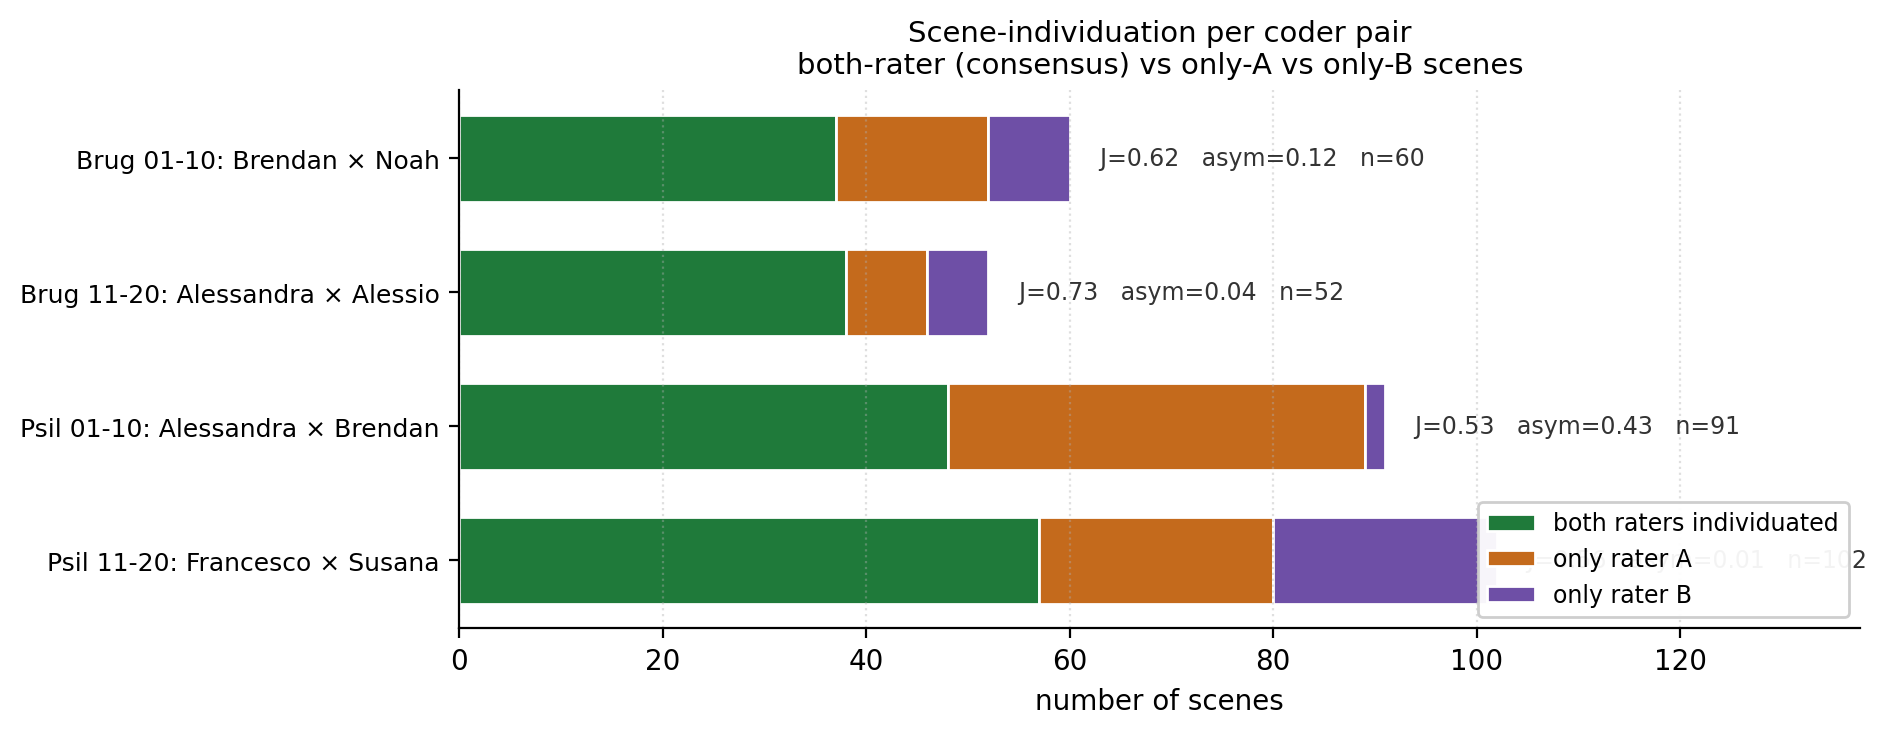
\includegraphics[width=0.97\linewidth]{figures/fig_R1_scene_individuation.png}
\caption{\textbf{Scene-individuation per coder pair.} Each horizontal bar shows the total union-individuation for one pair, segmented by whether both raters, only rater~A, or only rater~B pointed at that narrative passage as a hallucinatory scene. Jaccard (J), count asymmetry, and total $n$ are annotated to the right of each bar. The Alessandra~$\times$~Brendan pair (Psilocybe 01--10) is immediately visible as a threshold-mismatch outlier rather than a symmetric-disagreement pair: 41 of the 43 solo scenes come from rater~A and only 2 from rater~B.}
\label{fig:R1}
\end{figure}

Three pairs reach moderate-to-substantial Jaccard (0.56--0.73), a range consistent with reliable agreement on what counts as a discrete hallucinatory scene in trip reports written by independent authors for independent audiences. The fourth pair, Alessandra~$\times$~Brendan on Psilocybe 01--10, is not a case of symmetric disagreement but of threshold mismatch: Alessandra individuated 41 scenes Brendan did not, while Brendan individuated only 2 scenes Alessandra did not. The count-asymmetry index of 0.43 (Figure~\ref{fig:R1}) isolates this pair as the single largest contributor to Tier~1 disagreement in the corpus. The same pair also drives the lower aggregate Jaccard reported for psilocybin overall, and motivates the D1 (individuation-threshold mismatch) classification in \S\ref{sec:discrepancy-sources}.

Between substances, brugmansia pairs individuated more consistently (mean Jaccard $\approx$ 0.68) than psilocybin pairs ($\approx$ 0.55), consistent with brugmansia's characteristically concrete perceptual content (people, objects, insects, conversations) offering clearer scene boundaries than psilocybin's fractal, immersive, and metaphorical content. This differential, visible in the two bar groups of Figure~\ref{fig:R1}, foreshadows a substance-by-tier interaction that recurs at Tier~2.

\subsection{Attribute-classification reliability}
\label{sec:r-classification}

Restricted to the 180 AB scenes (both raters individuated), we computed, for each coder pair and each scene-level taxonomy item actually used by either rater on at least one AB scene, the $2\times 2$ agreement table and Cohen's $\kappa$, PABAK, and observed agreement (see \S\ref{sec:diagnostics}). Table~\ref{tab:attr-reliability} summarises the weighted means per coder pair.

\begin{table}[htbp]
\centering
\small
\begin{tabular}{lrrrrrl}
\toprule
Coder pair & AB scenes & items & obs.\ agr.\ $p_o$ & weighted $\kappa$ & PABAK & $\kappa$ label \\
\midrule
Psil.\ 11--20: Francesco $\times$ Susana    & 57 & 42 & 0.94 & 0.42 & 0.88 & moderate \\
Psil.\ 01--10: Alessandra $\times$ Brendan  & 48 & 41 & 0.94 & 0.34 & 0.89 & fair \\
Brug.\ 11--20: Alessandra $\times$ Alessio  & 38 & 31 & 0.91 & 0.31 & 0.81 & fair \\
Brug.\ 01--10: Brendan $\times$ Noah        & 37 & 26 & 0.92 & 0.17 & 0.83 & slight \\
\bottomrule
\end{tabular}
\caption{Attribute-classification reliability per coder pair, weighted across all scene-level items actually used on shared scenes. Cohen's $\kappa$ labels follow \citet{landis1977}. Observed agreement and PABAK are consistently $\ge 0.81$ across pairs (substantial--almost-perfect), whereas $\kappa$ spans slight to moderate --- a signature of the kappa paradox on low-prevalence leaves \citep{feinstein1990,byrt1993,sim2005}.}
\label{tab:attr-reliability}
\end{table}

Observed agreement is $\ge 0.91$ for every pair, and PABAK is in the substantial-to-almost-perfect range (0.81--0.89). Cohen's $\kappa$ nonetheless spans slight (0.17) to moderate (0.42). The discrepancy between $\kappa$ and the two base-rate-insensitive metrics reflects the prevalence structure of the taxonomy rather than a dispute about the data: most of the 147 taxonomy leaves are rare, tagged on only 1--3 of a pair's 37--57 AB scenes. At such prevalence extremes, $\kappa$ is known to drop sharply even when raters agree on nearly every case \citep{feinstein1990,sim2005}. Figure~\ref{fig:R2} illustrates the effect directly.

\begin{figure}[htbp]
\centering
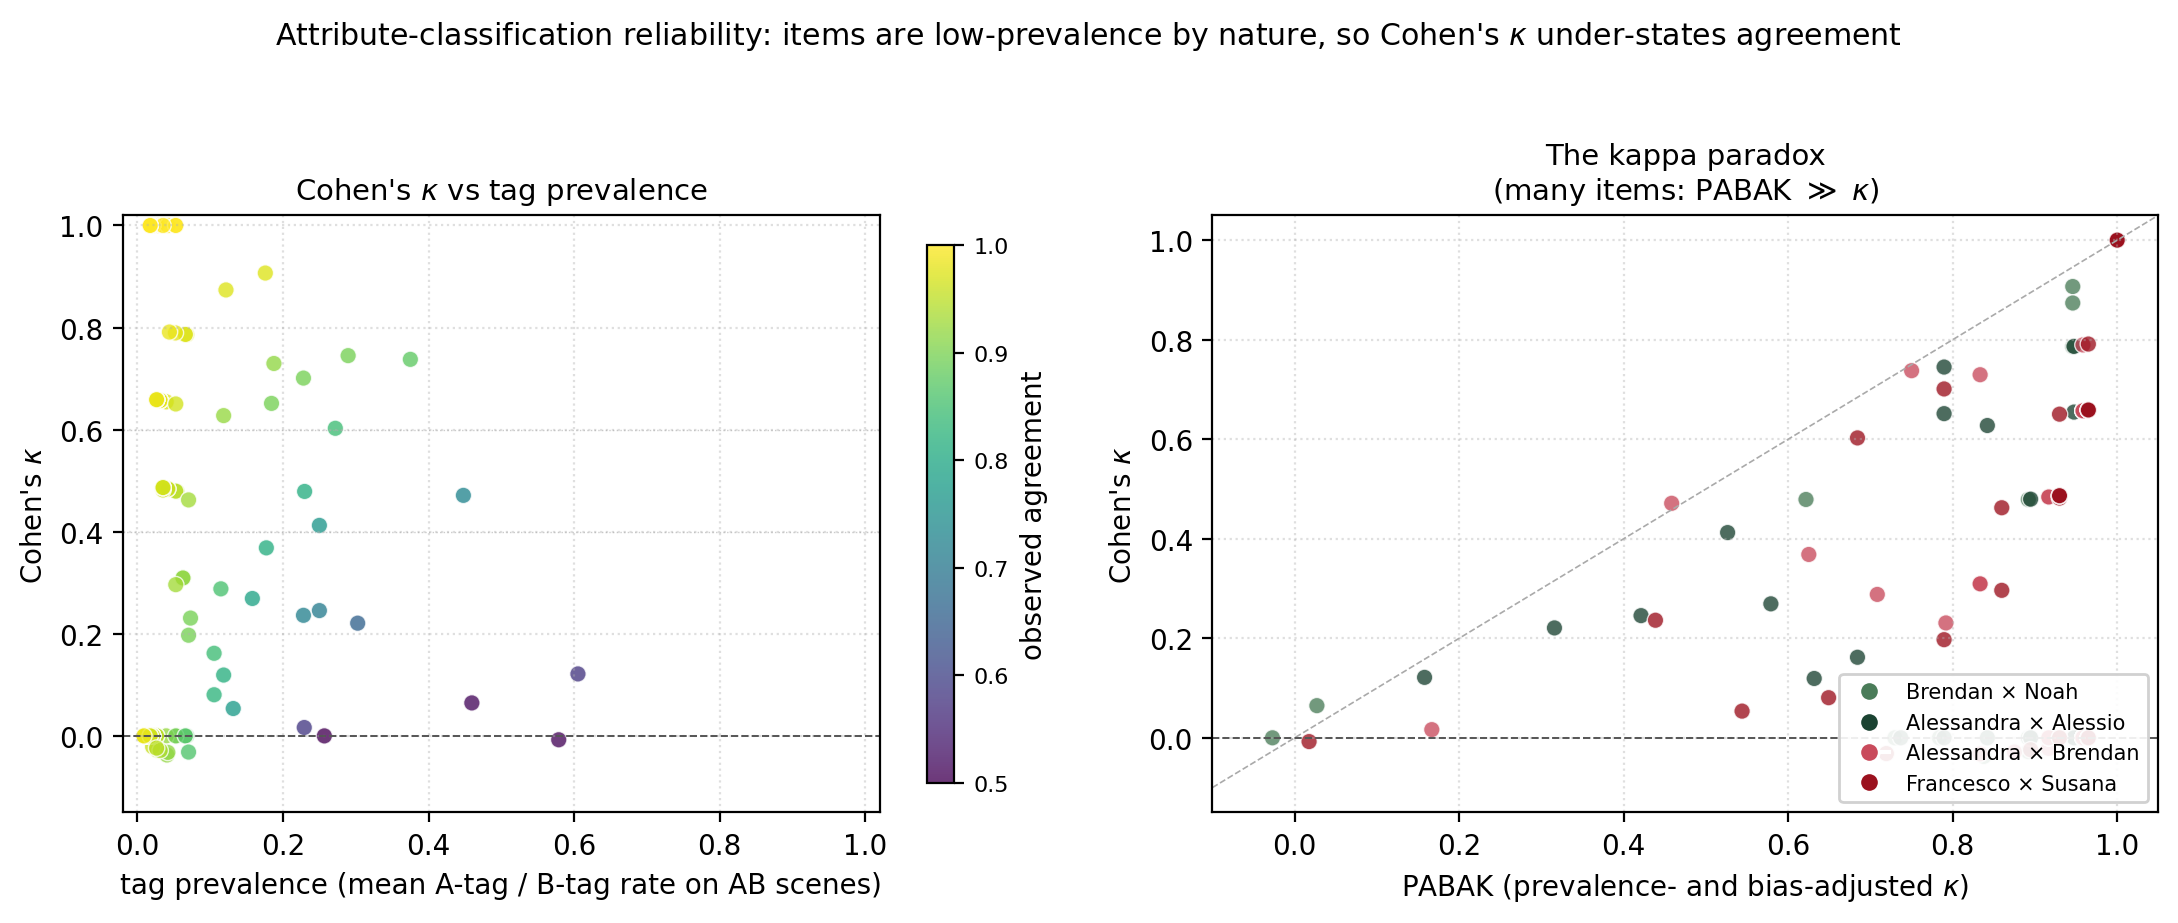
\includegraphics[width=0.99\linewidth]{figures/fig_R2_kappa_paradox.png}
\caption{\textbf{The kappa paradox on this dataset.} \emph{Left}: each point is one (coder-pair, taxonomy-item) combination; $x$ is the tag's prevalence (mean rater use rate on AB scenes), $y$ is Cohen's $\kappa$, colour is observed agreement. The mass at $\kappa \approx 0$ is concentrated on low-prevalence items despite observed agreement above 0.90 (dark-viridis). \emph{Right}: the same points plotted as $\kappa$ vs PABAK, coloured by coder pair; PABAK lies well above $\kappa$ for most items (below the dashed identity line), confirming that the low $\kappa$ values are prevalence artefacts, not evidence of unreliable coding. PABAK is therefore the more honest headline number for this taxonomy; we report Cohen's $\kappa$ alongside as the field-conventional figure.}
\label{fig:R2}
\end{figure}

Per-section structure is shown in the weighted-$\kappa$ heatmap in Figure~\ref{fig:R3}. Three patterns dominate. First, \emph{auditory hallucination} (mean $\kappa = 0.43$ across four pairs) and \emph{visual hallucination} (0.37) are the most reliable taxonomic sections: when raters agree that a sound or a visual object appeared, they agree on its rough character. Second, \emph{Type of visual alteration} (0.27) is reliably the noisiest high-prevalence section, driven in all four pairs by the \texttt{hallucination\_of\_a\_detached\_object} leaf: Alessandra~$\times$~Brendan, for example, tag it 20 vs 2 times on the 48 AB scenes of Psilocybe 01--10, and the pattern recurs at smaller magnitudes across the other three pairs. This aligns with the taxonomy-ambiguity source D2 identified in \S\ref{sec:discrepancy-sources}. Third, \emph{Modal status} (0.19) is the single least reliable section: on Psilocybe 11--20 both raters used the \texttt{impossible\_event} tag on 33 of 57 AB scenes, yet agreed on which 33 only 50.9\% of the time. Modal status is inherently a subjective classification of event plausibility and behaves as such; it is unlikely to be improved by Guidelines clarification alone.

\begin{figure}[htbp]
\centering
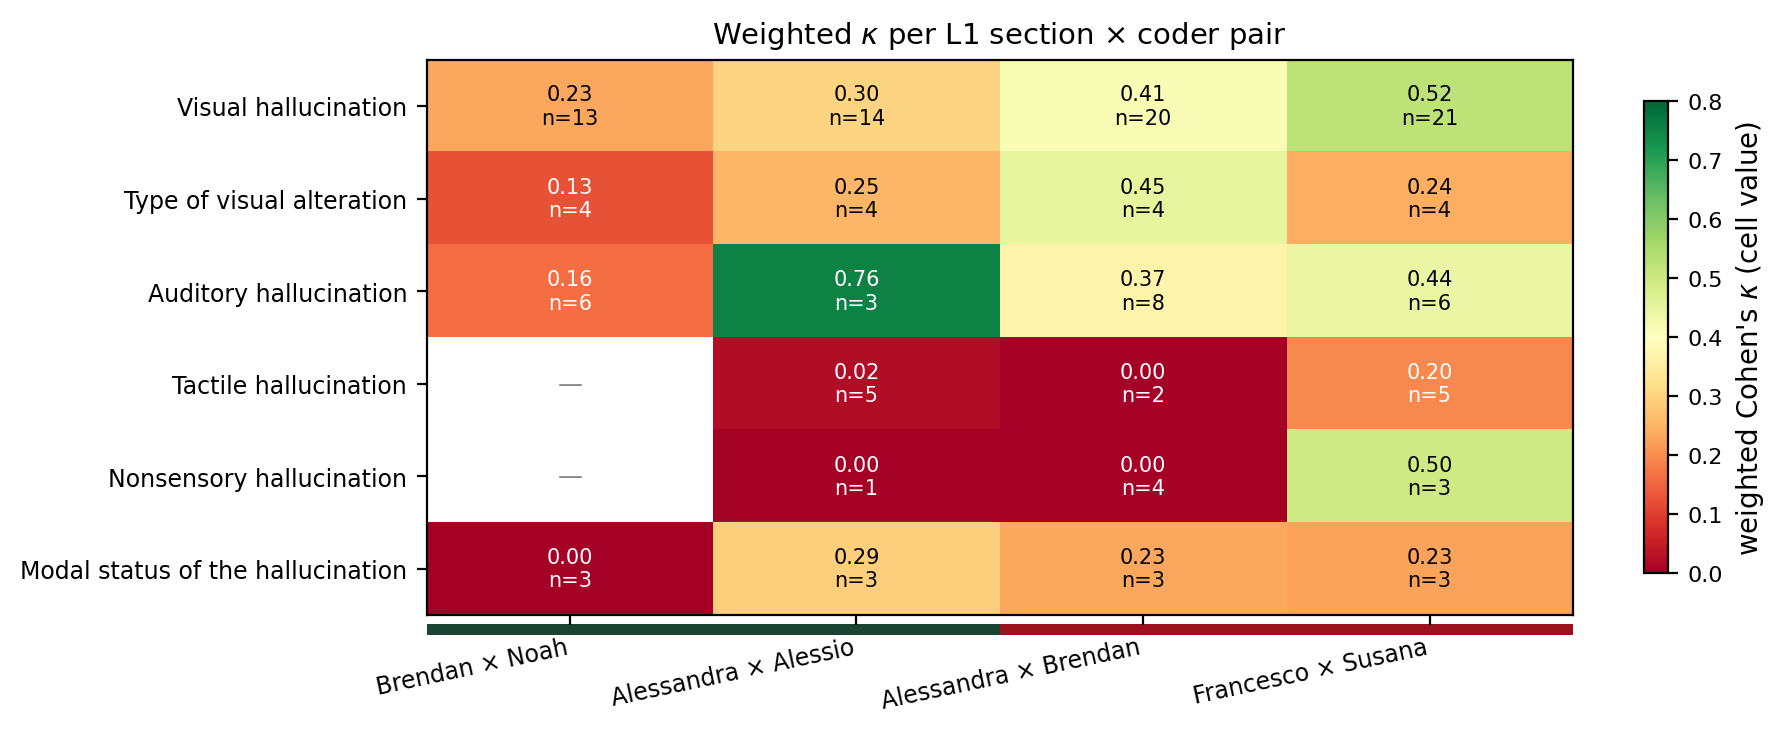
\includegraphics[width=0.97\linewidth]{figures/fig_R3_section_heatmap.png}
\caption{\textbf{Attribute-classification reliability by taxonomic section and coder pair.} Each cell is the $n_{\mathrm{shared\ scenes}}$-weighted mean Cohen's $\kappa$ across the items within a section that the pair actually used, with the number of active items annotated as $n{=}\cdot$. Em-dashes denote sections the pair did not use. Colour scale: RdYlGn 0.0--0.8. Auditory and Visual hallucination sections reach moderate reliability in every pair; \emph{Type of visual alteration} and \emph{Modal status} are uniformly weakest, implicating the taxonomy-ambiguity source D2.}
\label{fig:R3}
\end{figure}

Finally, the scene-centred view. For each AB scene we computed the Jaccard of the two raters' full tag sets, $J_s$ (see \S\ref{sec:diagnostics}). Figure~\ref{fig:R4} shows the resulting distribution split by substance. Median $J_s = 0.33$ in both substances: on a typical shared scene, raters agree on roughly one of every three tags they attached. The distribution is wide, with a substantial fraction of scenes at $J_s = 1.0$ (the two raters tagged the same small set exactly) and another at $J_s = 0.0$ (agreed a scene existed, disagreed on every tag). Psilocybin shows a slightly higher mean $J_s$ (0.42) than brugmansia (0.36), the reverse of the Tier~1 ordering and again consistent with the two substances differing in which tier of the coding decision is the rate-limiting step.

\begin{figure}[htbp]
\centering
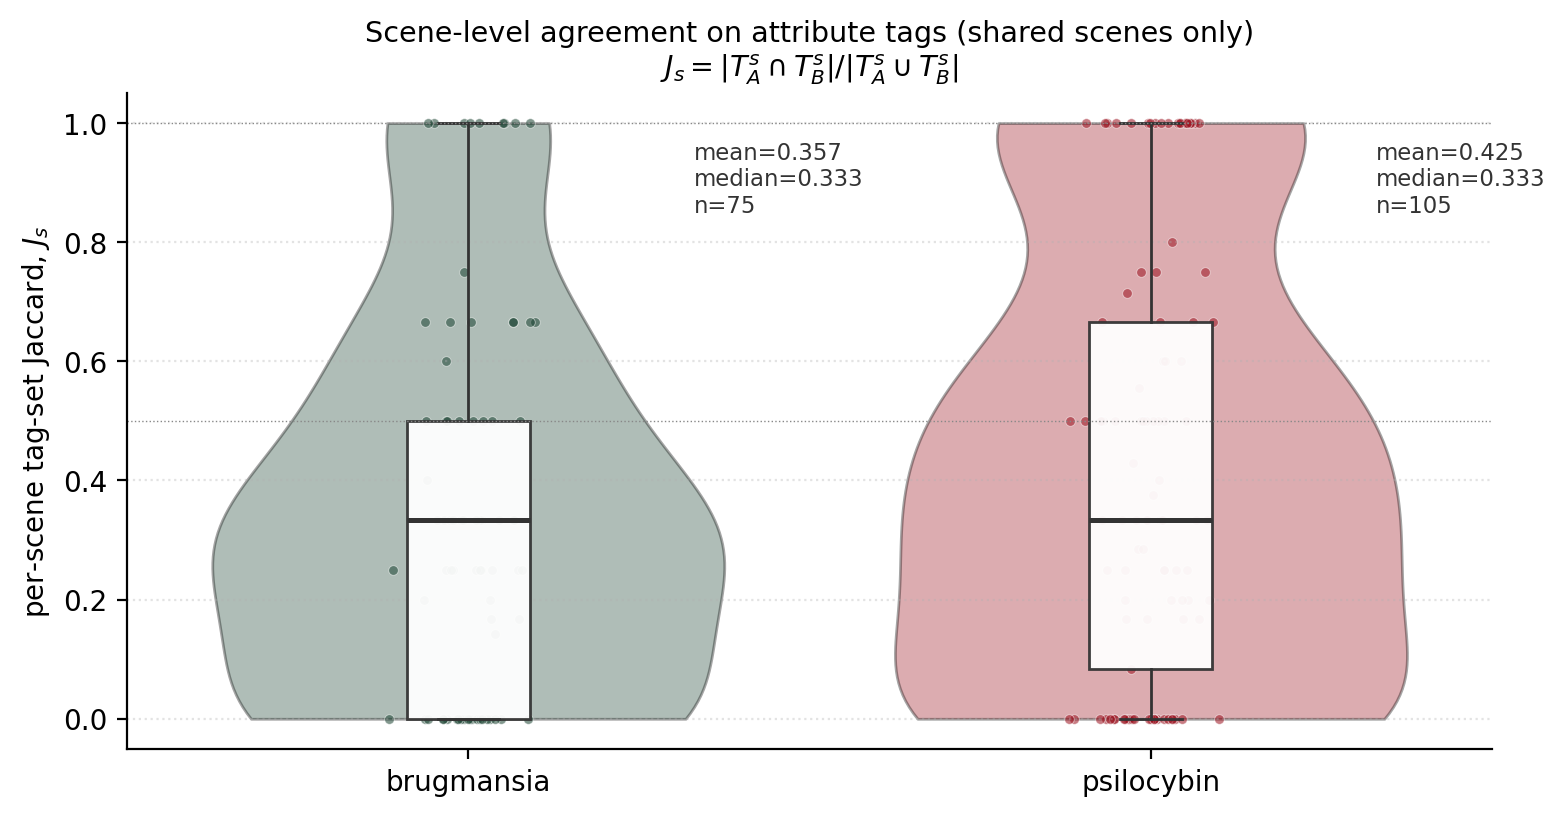
\includegraphics[width=0.85\linewidth]{figures/fig_R4_per_scene_jaccard.png}
\caption{\textbf{Per-scene tag-set Jaccard on shared scenes.} Violin (smoothed density) overlaid with a strip (each dot one AB scene) and an internal boxplot for both substances. Medians are identical (0.33) but distributions differ: brugmansia is bimodal with a concentration near $J_s{=}0.33$ and a secondary mode at $J_s{=}1.0$; psilocybin is more continuous. Means, medians, and $n$ are annotated inside the plot.}
\label{fig:R4}
\end{figure}

Taken together with the tier-1 results, Figures~\ref{fig:R1}--\ref{fig:R4} support the central methodological claim of this paper: agreement on \emph{whether a scene exists} is a separable, and substantially higher, quantity than agreement on \emph{how to classify it}. Both substances sit comfortably above chance at Tier~1 (Figure~\ref{fig:R1}); their Tier~2 profiles differ primarily in which taxonomic sections absorb the residual disagreement, with brugmansia concentrating its classification disagreement in the Type-of-visual-alteration axis and psilocybin in Modal status and the metaphor/inner-imagery leaves.

\subsection{Sources of rater discrepancy}
\label{sec:discrepancy-sources}

A systematic audit of the 40-trip recoded dataset (\texttt{1.Recoding/AUDIT\_AND\_MITIGATIONS.md}) identifies eight distinct sources of inter-rater discrepancy, ranked here by their contribution to the total 650 disagreement events in the dataset. Sources D1 and D3 jointly account for the majority of the signal; D2 is the principal residual source that cannot be resolved by dataset-level filtering alone.

\paragraph{D1. Individuation-threshold mismatch.}
The single dominant driver of individuation-level disagreement. Raters apply systematically different thresholds to the question of whether a narrative passage constitutes a discrete hallucinatory scene. Solo-scene counts by coder range from 6 (Alessio) to 49 (Alessandra), a 8$\times$ spread. The asymmetry is concentrated in the Psilocybin 01--10 pair, where Alessandra individuated 41 scenes her partner Brendan did not (a 20.5$\times$ within-pair asymmetry). Content systematically included only by the permissive raters --- brief perceptual amplifications (``everything glassy'', ``voices feel alien''), per-object fragments within already-shared scenes, metaphorical visionary content, and ambient colour changes --- falls into the Case-2 category of the project guidelines (\texttt{Guidelines.pdf \S5}), which the permissive raters treated as codable and the conservative raters did not.

\paragraph{D2. Taxonomy ambiguity in ``Type of visual alteration''.}
The principal driver of attribute-level disagreement and the stubbornest source overall. The four leaves in this section (illusion, hallucination of an incrusted object, hallucination of a detached object, full-blown immersive hallucination) are defined cleanly in the abstract but their boundaries are not disambiguated for realistic edge cases: amplified colour on a real object, breathing walls, closed-eye visionary worlds, and gradual morphing of real objects into hallucinated ones can reasonably carry two or more tags. On shared scenes, 65\% of taxonomy rows under this section are flagged \texttt{A\_ONLY} or \texttt{B\_ONLY} rather than \texttt{AGREE}.

\paragraph{D3. Stylistic tag over-use and under-use.}
Per-rater base-rate variation on specific taxonomy items drives many false-positive disagreement flags. Per-trip \texttt{Modal status} usage ranges from 0.1 per trip (Noah) to 5.9 per trip (Francesco), approximately 50$\times$. Similar but smaller asymmetries appear for the \texttt{Hallucination of an incrusted object} leaf. These are not semantic disagreements about content but procedural-discipline differences about which tags to reflexively attach.

\paragraph{D4. Scope-layer mismatch (scene-level vs trip-level).}
The same passage is coded scene-level by one rater and trip-level by the other. Recurring instances: delusional beliefs (``laws of physics had changed''), ego-dissolution experiences with imagery (``cosmic winds blew through the centre of where I had been''), anthropomorphised objects (``the play structure flipped me off''), and insight-imagery (``the universe as a mycelium''). The PDF taxonomy places \texttt{Sense of reality}, \texttt{Insight}, \texttt{Ego dissolution}, \texttt{Own body distortion} and \texttt{Domain-specific violation} at trip-level, but the instructions do not explicitly direct raters how to handle passages that also have a scene-level perceptual component.

\paragraph{D5. Per-object excerpt fragmentation style.}
Alessandra's coding practice included listing each distinct object class within a scene as a separate scene-level row (e.g.\ ``tree'', ``pine needles'', ``blue veins'' as three excerpts within one scene). This produced 66 scene-level excerpts for \texttt{Psilocybe\_02} alone versus 12 from Brendan covering the same content. This is a row-inflation style rather than a semantic disagreement; the PDF allows counting each object-class once per scene but does not prescribe a single-excerpt-per-item row structure.

\paragraph{D6. Lump-versus-split of evolving scenes.}
When a hallucinatory experience morphs over time (phase transitions within an NDE, repeated similar incidents, gradual evolution of a visionary world), some raters record one scene while others split the episode into phases. The PDF explicitly favours lumping --- ``a scene can change a little and still remains the same scene'' --- making splitting a minor rule deviation. In the current dataset only one case exhibited a clean lump--split pattern (\texttt{Brugmansia\_12\_S08}, retrofitted with the \texttt{LUMPA/SPLITB} convention); more latent cases likely exist but do not dominate the error budget.

\paragraph{D7. Somatic / interoceptive sensations coded as scenes.}
The PDF taxonomy places embodied phenomena (own-body distortion, arousal, ego-dissolution/bodily self) at trip-level. Susana systematically codes such passages (``de-animating into stone'', ``becoming a feather'', ``heartbeat irregularity'') as scene-level hallucinations, while her pair partner Francesco keeps them at trip-level. The PDF does not provide a scene-level equivalent for embodied content, so this is partly a taxonomy gap rather than a rater error.

\paragraph{D8. Cognitive insights and revelations coded as scenes.}
\texttt{Insight} is an explicit trip-level taxonomy item, but when an insight arrives accompanied by imagery (``the connection I visualised was a growing mycelium''), raters split on whether to code the passage at scene-level as a visual hallucination or at trip-level as existential insight. This overlaps with D4 but is specifically about insight-content with imagistic delivery.

\subsection{Mitigation: outcome of the conservative consensus filter}
% - After M6 scope-layer normalisation + M1 conservative consensus filter:
%   - 180 of 305 scenes retained (59\%)
%   - 229 of 754 attribute rows retained (30\%)
% - Table comparing headline distributions of each major taxonomy section
%   in the pre-filter vs post-filter datasets, to show what content the
%   consensus view preserves and what it drops.

\subsection{Phenomenological profile of psilocybin}
% Consensus-filtered scene and attribute frequencies.
% - dominant alteration type
% - dominant object classes in visual hallucinations
% - auditory / tactile / nonsensory modality frequencies
% - emotion and insight profiles
% - ego dissolution frequencies

\subsection{Phenomenological profile of brugmansia}
% same structure

\subsection{Direct comparison}
% - items significantly more frequent in one substance than the other
% - qualitatively characteristic differences:
%   - psilocybin: geometric patterns, ego dissolution, metaphysical insight, extraordinary entities
%   - brugmansia: incrusted object hallucinations of humans/acquaintances,
%     delusional belief states, amnesia
% - scene-individuation rates per substance (are brugmansia trips more
%   hallucination-dense than psilocybin trips per word, etc.)
